% Sources: report/sections/03a_method_unet.md (Janu, #3), 03b_method_pretrained.md (Trivedh, #4),
% 03c_method_attention_transformer.md (Debangsu, #5).
\section{Method}
\label{sec:method}

\subsection{U-Net baseline and training setup}
\label{sec:unet}

\paragraph{Architecture.}
Our baseline is the U-Net of Ronneberger \etal~\cite{ronneberger2015unet}, an encoder--decoder network shaped like the letter U.
\begin{itemize}
  \item \textbf{Encoder (contracting path).} Five levels, each a \emph{double convolution}: two $3\times3$ convolutions, each
        followed by batch normalisation and a ReLU. The number of channels doubles at every level:
        $64 \rightarrow 128 \rightarrow 256 \rightarrow 512 \rightarrow 1024$. Between levels, a $2\times2$ max-pooling halves the height and width, so a
        $352\times352$ input becomes 176, 88, 44 and finally \textbf{$22\times22$} pixels at the deepest level. Deeper levels see a
        larger part of the image and learn \emph{what} is in it, but they lose \emph{where} exactly it is.
  \item \textbf{Decoder (expanding path).} Four steps. Each step uses a $2\times2$ transposed convolution to double the
        resolution and halve the channels, then a double convolution, until the output is $352\times352$ again.
  \item \textbf{Skip connections.} Before each decoder double convolution, the decoder feature map is
        \textbf{concatenated with the encoder feature map of the same resolution}. This brings back the fine spatial
        detail (polyp edges) that pooling discarded, and is the key idea of U-Net.
  \item \textbf{Output.} A final $1\times1$ convolution maps the 64 channels to \textbf{one logit per pixel}. A sigmoid turns the
        logit into the probability that the pixel belongs to a polyp; pixels above a threshold (0.5 unless stated
        otherwise) form the predicted mask.
\end{itemize}
We make two common changes to the original design. First, we add \textbf{batch normalisation} after every
convolution, which makes training from scratch faster and more stable. Second, we use \textbf{padded convolutions},
so the output has the same size as the input. The original U-Net used unpadded convolutions and had to crop
the skip connections. Our U-Net has \textbf{31.0 million parameters}.

\paragraph{Loss function.}
The loss is the sum of two terms:
\begin{equation}
  \mathcal{L} = \mathrm{BCE}(p, g) + \bigl(1 - \mathrm{Dice}(p, g)\bigr),
  \label{eq:loss}
\end{equation}
where $p$ are the predicted probabilities and $g$ is the ground-truth mask.
\begin{itemize}
  \item \textbf{Binary cross-entropy (BCE)} scores every pixel independently and gives smooth, stable gradients.
  \item \textbf{Soft Dice loss} scores the overlap between the whole predicted polyp and the true polyp. Polyps often
        cover less than 20\% of the image, so a model trained with BCE alone can reach a low loss by predicting
        ``background'' almost everywhere. The Dice term prevents this, because it is computed only from the polyp
        pixels.
\end{itemize}

\paragraph{Optimisation.}
\begin{itemize}
  \item \textbf{AdamW} (learning rate $3\cdot10^{-4}$, weight decay $10^{-4}$), batch size 8.
  \item \textbf{OneCycle learning-rate schedule:} the learning rate rises during the first 10\% of the steps (warm-up),
        then decays following a cosine curve, which gives stable early training and a fine final convergence.
  \item \textbf{60 epochs} of 100 steps each (800 images / batch 8).
  \item \textbf{Mixed precision (fp16)} on the GPU, which roughly halves memory use and speeds up training.
        The loss itself is computed in fp32 for numerical stability.
  \item \textbf{Model selection:} after every epoch we compute the Dice score on the validation set and keep the weights
        of the best epoch. The test set plays no part in this choice.
  \item A fixed random seed (42) controls the weight initialisation and the augmentation, so a rerun gives
        nearly the same model (some GPU operations are not bit-exact between runs).
\end{itemize}
Training the baseline took 46 minutes on an NVIDIA T4 GPU (60 epochs). The best validation Dice, 0.855,
was reached at epoch 54; by the last epoch it was still 0.852, so the model had converged without
overfitting the validation set.

\paragraph{Evaluation metrics.}
For each test image we compare the predicted mask $P$ with the ground truth $G$ and count true positive
(TP), false positive (FP) and false negative (FN) pixels:
\begin{align}
  \mathrm{Dice} &= \frac{2\,\mathrm{TP}}{2\,\mathrm{TP} + \mathrm{FP} + \mathrm{FN}} = \frac{2\,|P \cap G|}{|P| + |G|}, \label{eq:dice}\\
  \mathrm{IoU}  &= \frac{\mathrm{TP}}{\mathrm{TP} + \mathrm{FP} + \mathrm{FN}} = \frac{|P \cap G|}{|P \cup G|}, \label{eq:iou}\\
  \mathrm{Precision} &= \frac{\mathrm{TP}}{\mathrm{TP} + \mathrm{FP}}, \qquad
  \mathrm{Recall} = \frac{\mathrm{TP}}{\mathrm{TP} + \mathrm{FN}}.
\end{align}
IoU is the Jaccard index. Precision measures how much of the prediction is really polyp, and recall how much of the polyp was found.
Each metric is computed \textbf{per image and then averaged} over the 120 test images, so a small polyp counts as
much as a large one. Dice is always at least as large as IoU for the same prediction
($\mathrm{Dice} = 2\,\mathrm{IoU} / (1 + \mathrm{IoU})$).

\paragraph{Baseline result.} On the test set, the U-Net trained from scratch reaches a \textbf{Dice of 0.851} and an
\textbf{IoU of 0.774} (precision 0.867, recall 0.897). This is the reference point for every other model in \cref{sec:results}.

\subsection{Pretrained encoders: ResNet-34 and MobileNetV2}
\label{sec:pretrained}

\paragraph{Why pretrain the encoder.}
Kvasir-SEG has only 800 training images, far too few to teach a U-Net encoder to recognise edges,
textures and shapes from scratch (\cref{sec:unet}'s \texttt{unet\_scratch} has to learn all of that from polyp images
alone). Transfer learning swaps the encoder for one already trained on ImageNet's 1.2 million natural
images: it starts out already knowing general-purpose visual features, and only has to adapt them to
colonoscopy images and learn the decoder from zero. This is the standard fix for small medical-imaging
datasets, where collecting and labelling more data is expensive. Both encoders below come from
\texttt{segmentation\_models\_pytorch}, which attaches a U-Net decoder (same skip-connection design as \cref{sec:unet})
to a pretrained backbone.

\paragraph{ResNet-34 encoder (\texttt{unet\_resnet34}).}
Built with \texttt{smp.Unet("resnet34", encoder\_weights="imagenet")}. ResNet-34's residual blocks add the input
of a block back onto its output ($y = F(x) + x$) instead of only passing it through convolutions. This
shortcut lets gradients flow directly through the skip path during backpropagation, which is what makes
very deep encoders like this one trainable at all, and is also why its ImageNet features transfer well: the
network can reuse early, general-purpose filters almost unchanged while later layers specialise. At
\textbf{24.4\,M parameters} it is smaller than the from-scratch baseline (31.0\,M, \cref{sec:unet}) even though it is
deeper, because its widest layers have 512 channels instead of 1024 (the baseline's 1024-channel bottleneck,
in the \texttt{UNet} class in \texttt{common.py}, alone holds about 14\,M parameters), and the \texttt{smp} decoder
($256 \rightarrow 16$ channels) is lighter than ours ($512 \rightarrow 64$).

\paragraph{MobileNetV2 encoder (\texttt{unet\_mobilenetv2}).}
Built with \texttt{smp.Unet("mobilenet\_v2", encoder\_weights="imagenet")}. MobileNetV2 replaces each standard $3\times3$
convolution with a \textbf{depthwise-separable} block: a $3\times3$ convolution applied one channel at a time
(depthwise), followed by a $1\times1$ convolution that mixes channels (pointwise). A standard $3\times3$ convolution over
$C$ channels costs $9C^2$ multiply-adds per pixel; the depthwise-separable version costs $9C + C^2$, roughly
\textbf{8--9$\times$ fewer operations} for the channel counts used here. This is the encoder that trades some accuracy for
speed, at only \textbf{6.6\,M parameters}, about a quarter of ResNet-34's size and a fifth of the baseline's. It
is our candidate for a model light enough to run in real time (\cref{sec:speed}).

\paragraph{Training setup.}
Both models train for \textbf{40 epochs}, fewer than the baseline's 60, because a pretrained encoder already
starts close to a good solution and converges faster: most of the remaining learning is in the decoder and
in adapting the encoder to this domain, not in re-learning low-level features. Only ResNet-34 uses a
learning rate lower than the baseline's: \textbf{$2\cdot10^{-4}$}, which keeps the early optimisation steps from making
large updates to the pretrained weights before the new decoder has learned anything useful; large early
updates would otherwise erase the ImageNet features before they can help. MobileNetV2 trains stably at the
baseline's own \textbf{$3\cdot10^{-4}$}, so it keeps that rate unchanged. Loss, optimiser (AdamW), schedule (OneCycle),
batch size and evaluation metrics are unchanged from \cref{sec:unet}.

On the test set, \texttt{unet\_resnet34} reaches a \textbf{Dice of 0.903} (IoU 0.846) and \texttt{unet\_mobilenetv2} reaches a
\textbf{Dice of 0.894} (IoU 0.835), both well above the from-scratch baseline's 0.851, confirming that ImageNet
pretraining helps substantially on this small dataset even though the source images (natural photos) look
nothing like colonoscopy frames. The full comparison across all five models is in \cref{sec:results}.

\subsection{Attention U-Net}
\label{sec:attention}

\paragraph{Idea.}
A plain U-Net copies every encoder feature into the decoder through its skip connections, including
features from folds, glare, instruments and on-screen text. The Attention U-Net of Oktay \etal~\cite{oktay2018attention}
adds an \textbf{attention gate} to each skip connection, which learns \textbf{where to look}: it gives every pixel
of the skip feature a weight between 0 and 1, so background is suppressed before the decoder uses it.

\paragraph{Attention gate.}
For one skip connection, let
\begin{itemize}
  \item $x$ be the encoder skip feature map. It has fine resolution and knows \emph{where} the edges are.
  \item $g$ be the decoder feature map at the same resolution, just after upsampling. It comes from deeper in
        the network and carries the context of \emph{what} a polyp looks like.
\end{itemize}
The gate computes one attention coefficient per pixel:
\begin{equation}
  \alpha = \sigma\bigl(\psi(\mathrm{ReLU}(W_g\, g + W_x\, x))\bigr), \qquad \text{output} = x \cdot \alpha .
  \label{eq:gate}
\end{equation}
\begin{itemize}
  \item $W_g$ and $W_x$ are $1\times1$ convolutions (each followed by batch normalisation) that project $g$ and $x$
        into a shared space with half as many channels as $x$.
  \item Adding the two projections and applying ReLU keeps a location only where both the context ($g$) and the
        local detail ($x$) respond.
  \item $\psi$ is a $1\times1$ convolution down to \textbf{one channel}, and $\sigma$ is the sigmoid, so $\alpha \in [0, 1]$ at every pixel.
  \item The gated skip $x \cdot \alpha$ replaces $x$ in the concatenation. Pixels with $\alpha \approx 0$ contribute almost nothing.
\end{itemize}

\paragraph{Where the gates sit.}
The network is \textbf{identical to the baseline U-Net} of \cref{sec:unet} ($64 \rightarrow 1024$ channels, trained from scratch,
BCE + Dice loss, AdamW, learning rate $3\cdot10^{-4}$, 60 epochs, OneCycle schedule, seed 42). The only change is
one gate on each of the four skip connections, at \textbf{$44\times44$, $88\times88$, $176\times176$ and $352\times352$ pixels} (gates 1 to 4,
from the deepest to the shallowest). The gates add only 0.35\,M parameters (31.4\,M in total, +1.1\%), so any
difference from the baseline comes from the gates themselves.
Training took 54 minutes on an NVIDIA T4. The best validation Dice, 0.859, was reached at epoch 47.

\paragraph{Result.}
On the test set the Attention U-Net reaches a \textbf{Dice of 0.854} and an \textbf{IoU of 0.775}
(precision 0.868, recall 0.895), against 0.851 / 0.774 for the baseline. The gain of \textbf{+0.003 Dice is
too small to be meaningful} from a single training run. With test-time augmentation it scores 0.857 (baseline 0.863), and on the unseen
CVC-ClinicDB data 0.741 (baseline 0.750). \textbf{On Kvasir-SEG, attention gates do not measurably improve a U-Net
trained from scratch.} A likely reason is that the baseline already learns to ignore most background through
its decoder, and 800 training images are not enough for the extra gating to pay off.

\paragraph{Attention maps.}
\Cref{fig:attention} shows $\alpha$ for each gate on four test images, ordered from the smallest
polyp (0.5\% of the image) to the largest (71.9\%). Red means $\alpha$ close to 1 and blue means $\alpha$ close to 0.
\begin{itemize}
  \item \textbf{Gate 1 (44\,px)} is coarse and noisy. At this depth $\alpha$ marks broad regions rather than the polyp.
  \item \textbf{Gates 2 and 3 (88 and 176\,px)} trace the \textbf{polyp boundary}: for the 7.8\% and 17.8\% polyps they draw a
        clear ring around the lesion. They mostly pass edge information, which is what the skip connections are
        for.
  \item \textbf{Gate 4 (352\,px)} highlights the \textbf{polyp body} of the medium polyps and keeps much of the background low.
  \item \textbf{Where the gates help and where they hurt.} The per-image test Dice of these images shows both sides.
        For the \textbf{tiny 0.5\% polyp}, the maps are diffuse, but gate 3 shows a small ring at the lesion. The
        Attention U-Net reaches a Dice of \textbf{0.593 against 0.129} for the baseline, its clearest gain.
        For the \textbf{71.9\% polyp}, the gates highlight only part of it, because a lesion that fills the frame looks
        like background tissue. Dice falls to \textbf{0.573 against 0.781} for the baseline.
        The gates also respond to \textbf{on-screen text and the black overlay box} in the corner. These artefacts are
        common in Kvasir-SEG, and $\alpha$ does not learn to ignore them.
\end{itemize}
These opposite effects on small and very large polyps largely cancel out, which explains why the average
Dice barely changes.

\begin{figure*}[t]
  \centering
  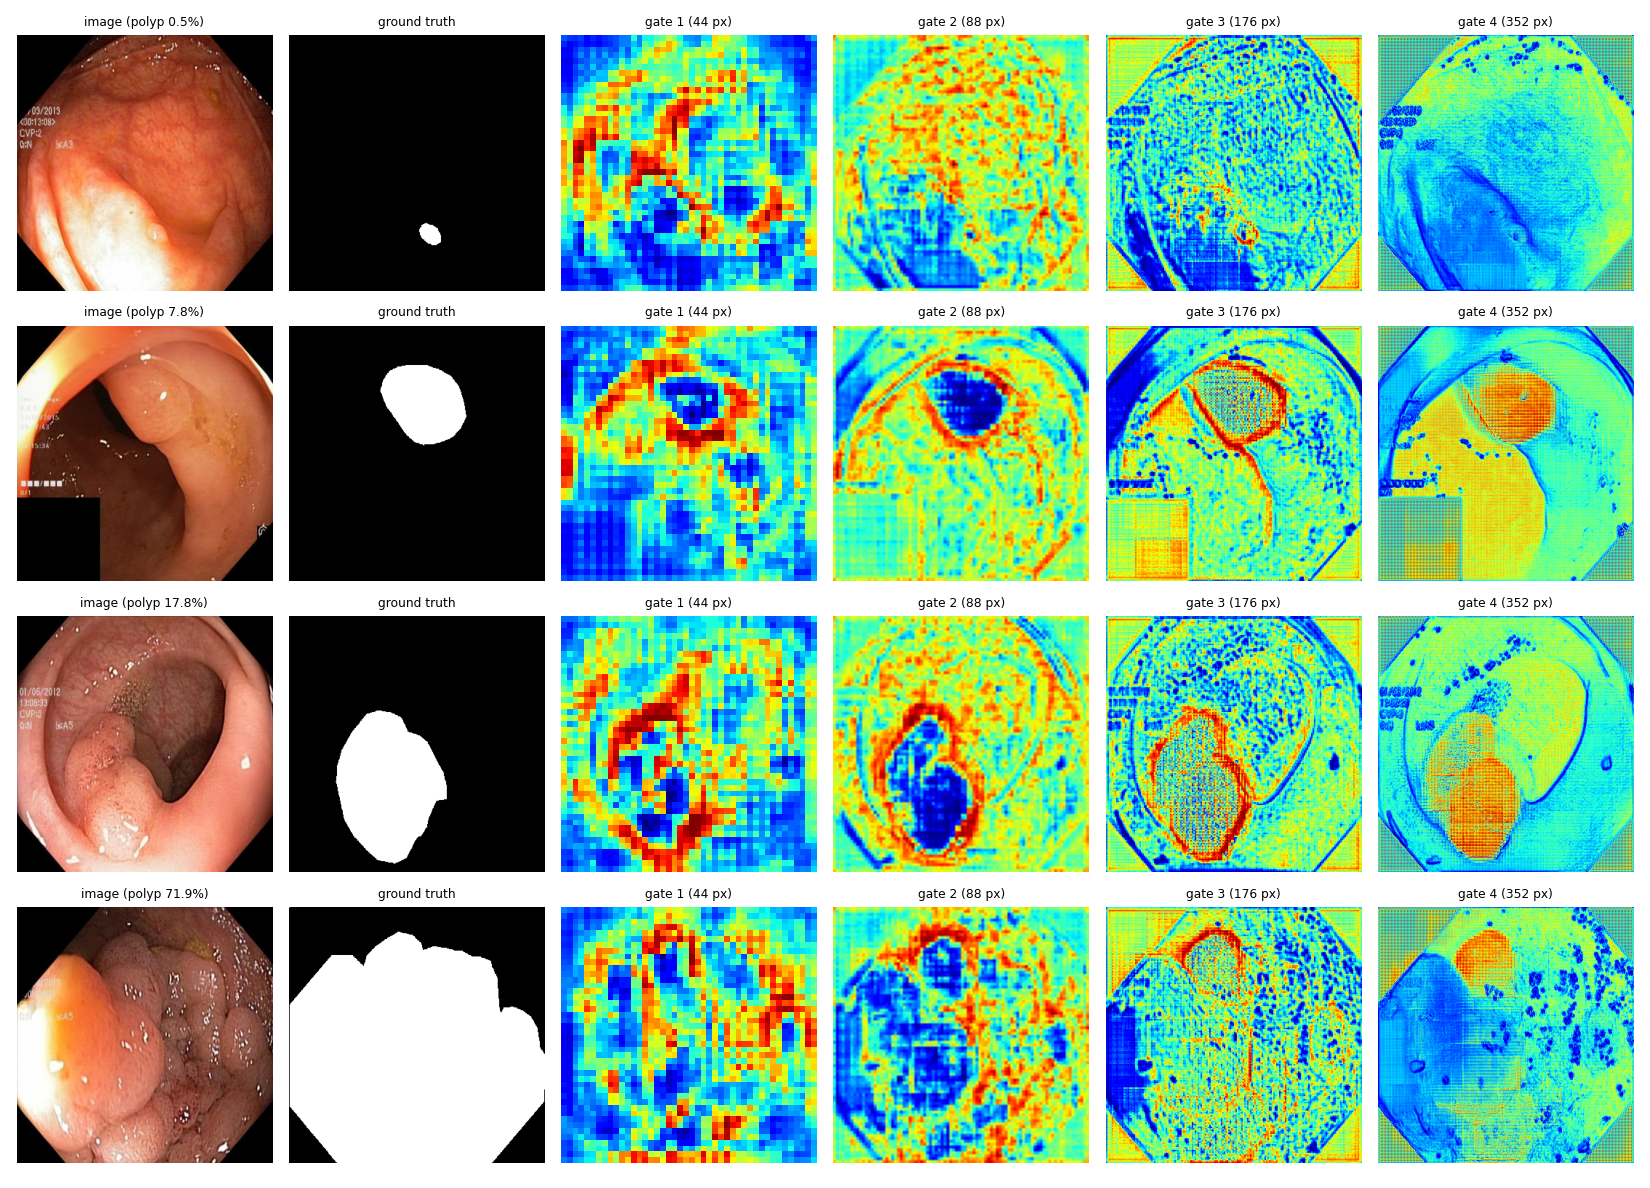
\includegraphics[width=0.86\textwidth]{attention_maps.png}
  \caption{Attention coefficients $\alpha$ of the four gates of the Attention U-Net on four test images (red: $\alpha$ close to 1, blue: $\alpha$ close to 0).}
  \label{fig:attention}
\end{figure*}

\subsection{SegFormer (MiT-B2 transformer encoder)}
\label{sec:segformer}

\paragraph{Encoder: hierarchical transformer.}
SegFormer~\cite{xie2021segformer} replaces the convolutional encoder with a \textbf{Mix Transformer (MiT-B2)}.
\begin{itemize}
  \item The image is cut into \textbf{overlapping patches} (a strided convolution), so neighbouring patches share pixels.
        Positional information comes from \textbf{Mix-FFN}, a $3\times3$ depthwise convolution inside each feed-forward layer,
        so no positional embedding is needed and the model works at any input size.
  \item Each transformer block applies \textbf{self-attention}: every patch compares itself with every other patch and
        takes a weighted average of them. Every location can therefore use the \textbf{whole image as context}, while a
        CNN only sees a local window that grows slowly with depth. To keep this affordable at high resolution,
        MiT uses \emph{efficient} self-attention, which shrinks the keys and values by a fixed ratio.
  \item Four stages produce features at \textbf{1/4, 1/8, 1/16 and 1/32} of the input size (88, 44, 22 and 11 pixels for
        a $352\times352$ image), a multi-scale pyramid like a CNN's.
\end{itemize}

\paragraph{Decoder: all-MLP.}
The decoder is deliberately light. Each of the four feature maps is projected to the same number of channels
by an MLP (a $1\times1$ convolution), upsampled to 1/4 resolution, concatenated, fused by one more MLP, and mapped to
one logit per pixel. The prediction is made at \textbf{$88\times88$}, and the segmentation head \textbf{bilinearly upsamples} it
$\times4$ to $352\times352$ before the loss and metrics. (Our \texttt{Resize} wrapper would resize any other output to the input
size, but here it is only a safety net and never changes the output.)

\paragraph{Training setup.}
\begin{itemize}
  \item Encoder initialised with \textbf{ImageNet-pretrained} MiT-B2 weights (\texttt{segmentation-models-pytorch} 0.6.0).
  \item The same loss, augmentation, split, batch size, optimiser and schedule as the U-Nets, except
        \textbf{40 epochs} and a \textbf{learning rate of $10^{-4}$}. Transformers are sensitive to large learning rates, which
        would destroy the pretrained weights.
  \item 24.7\,M parameters. Training took only 12 minutes on an NVIDIA T4. The best validation Dice, 0.913, was
        reached at epoch 23.
\end{itemize}

\paragraph{Result.}
SegFormer is the strongest model so far:
\textbf{Dice 0.917} and \textbf{IoU 0.865} on the test set (precision 0.911, recall 0.943), \textbf{+0.066 Dice} over the
baseline, with fewer parameters; 0.926 with test-time augmentation; and
\textbf{0.863 on CVC-ClinicDB}, against 0.750 for the baseline. The gap is largest on the unseen dataset, which
suggests that global context and ImageNet pretraining help the model generalise to a new hospital.

\subsection{Threshold tuning}
\label{sec:threshold}
The models output a probability per pixel, and by default a pixel is called ``polyp'' when $p > 0.5$.
That value is a convention, not necessarily the best choice. We tune it as follows:
\begin{enumerate}
  \item On the \textbf{validation set only}, compute the mean Dice for the thresholds $0.20, 0.25, \dots, 0.80$.
  \item Keep the threshold with the highest validation Dice (\texttt{thr\_val}).
  \item Apply it \textbf{once} to the test set (\texttt{dice\_tuned}).
\end{enumerate}
Choosing the threshold on the test set would leak test information into the model and over-state the score.
The test set must stay unseen until the final evaluation.

\begin{figure}[t]
  \centering
  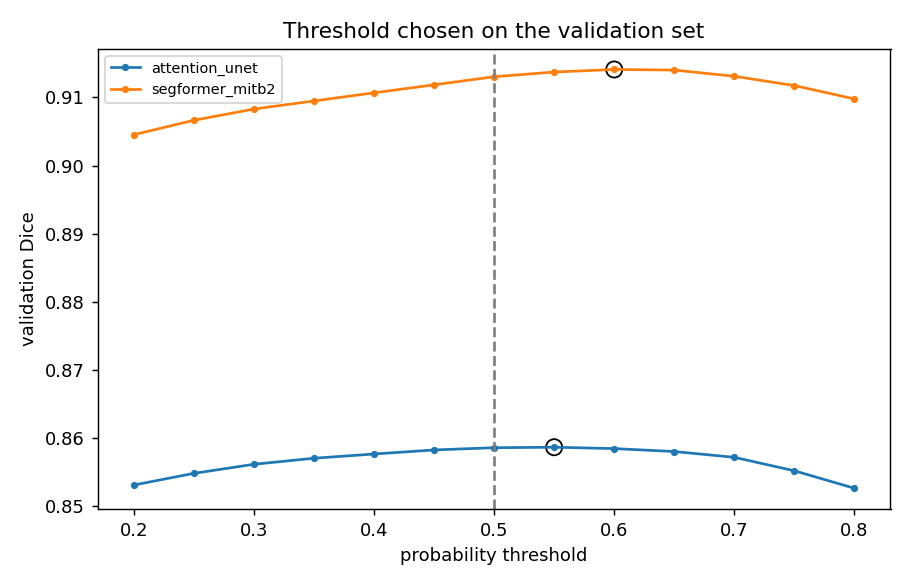
\includegraphics[width=\linewidth]{threshold_curve.png}
  \caption{Validation Dice against the probability threshold.}
  \label{fig:threshold}
\end{figure}

\begin{table}[t]
  \centering
  \small
  \setlength{\tabcolsep}{4pt}
  \begin{adjustbox}{max width=\linewidth}
  \begin{tabular}{@{}lcccc@{}}
    \toprule
    Model & Best thr.\ (val) & Dice at 0.5 & Dice tuned & Gain \\
    \midrule
    U-Net baseline   & 0.50 & 0.851 & 0.851 & 0.000 \\
    Attention U-Net  & 0.55 & 0.854 & 0.854 & +0.0007 \\
    SegFormer MiT-B2 & 0.60 & 0.917 & 0.918 & +0.0008 \\
    \bottomrule
  \end{tabular}
  \end{adjustbox}
  \caption{Threshold chosen on the validation set and its effect on test Dice.}
  \label{tab:threshold}
\end{table}

Both curves in \cref{fig:threshold} are \textbf{flat around 0.5}: between 0.4 and 0.7, validation Dice
varies by only 0.0015 for the Attention U-Net and 0.0034 for SegFormer. The chosen thresholds sit just above
0.5, so the models are slightly better when they mark a pixel as polyp only when they are a little more
confident. The gain is \textbf{about +0.001 Dice (+0.0007 and +0.0008)} (\cref{tab:threshold}), so threshold tuning is not a meaningful
source of improvement here.

The flat curves show instead that the models' predictions are \textbf{confident (sharp)}: most pixels are
predicted close to 0 or 1. On the test set, only \textbf{3.0\%} (Attention U-Net) and \textbf{2.2\%} (SegFormer) of
pixels have a probability between 0.2 and 0.8, so moving the threshold changes very few of them, and the
default of 0.5 is a safe choice. This is not the same as \emph{calibration}, which would mean that pixels
predicted at, say, 0.8 are polyp 80\% of the time. We did not measure calibration.
